%%%%%%%%%%%%%%%%%%%%%%%%%%%%%%%%%%%%%%%%%
% Beamer Presentation
% LaTeX Template
% Version 1.0 (10/11/12)
%
% This template has been downloaded from:
% http://www.LaTeXTemplates.com
%
% License:
% CC BY-NC-SA 3.0 (http://creativecommons.org/licenses/by-nc-sa/3.0/)
%
%%%%%%%%%%%%%%%%%%%%%%%%%%%%%%%%%%%%%%%%%

%----------------------------------------------------------------------------------------
%	PACKAGES AND THEMES
%----------------------------------------------------------------------------------------

\documentclass{beamer}

\mode<presentation> {

\usetheme{Madrid}

}

\usepackage{graphicx} % Allows including images
\usepackage{booktabs} % Allows the use of \toprule, \midrule and \bottomrule in tables
\usepackage{tikz}
%----------------------------------------------------------------------------------------
%	TITLE PAGE
%----------------------------------------------------------------------------------------

\title[Gallai Colorings and S-rings]{Gallai Colorings of Complete
  Graphs With Applications to the Theory of S-rings} % The short title appears at the bottom of every slide, the full title is only on the title page

\author[Bruce Chiarelli]{Bruce Chiarelli \and Dr. Stephen Humprhies} % Your name
\institute[BYU] % Your institution as it will appear on the bottom of every slide, may be shorthand to save space
{
Brigham Young University \\ % Your institution for the title page
}
\date{February 28, 2014} % Date, can be changed to a custom date

\begin{document}

\begin{frame}
\titlepage % Print the title page as the first slide
\end{frame}


\begin{frame}
\frametitle{Permutations}
\begin{block} {Definition}
\begin{itemize}
\item A \emph{permutation} is an ordered arrangement of objects. 
\pause
\item In this presentation, a permutation will be considered as a
  function that rearranges a given collection of objects.
\end{itemize}
\end{block}
\pause
Example: 
\begin{columns}
\column{.4\textwidth}
\begin{figure}
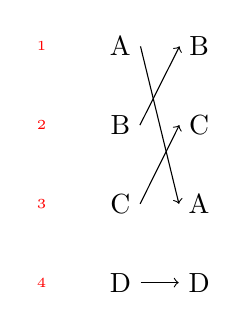
\begin{tikzpicture}
\node (a1) {A};
\node (b1) [below of = a1] {B};
\node (c1) [below of = b1] {C};
\node (d1) [below of = c1] {D};
\pause
\node (b2) [right of = a1] {B};
\node (c2) [right of = b1] {C};
\node (a2) [right of = c1] {A};
\node (d2) [right of = d1] {D};
\draw[->] (a1.east) -- (a2.west);
\draw[->] (b1.east) -- (b2.west);
\draw[->] (c1.east) -- (c2.west);
\draw[->] (d1.east) -- (d2.west);
\pause
\onslide<5-> {
\node (a0) [left of = a1,text=red] {\tiny 1};
\node (b0) [left of = b1,text=red] {\tiny 2};
\node (c0) [left of = c1,text=red] {\tiny 3};
\node (d0) [left of = d1,text=red] {\tiny 4};
}
\end{tikzpicture}
\end{figure}
\column{.4\textwidth}
\begin{itemize}
\onslide<5->{
\item We will use this notation:
$$ \left(\begin{tabular}{cccc}
1 & 2 & 3 & 4 \\
3 & 1 & 2 & 4 \\
\end{tabular}\right) $$ or $$ \left(\begin{tabular}{ccc}
1 & 2 & 3 \\
3 & 1 & 2 \\
\end{tabular}\right)$$ }
\end{itemize}
\end{columns}
\end{frame}

\begin{frame}
\frametitle{Transpositions}
\begin{block}{Definition}
\begin{itemize}
\item A \emph{transposition} is a permutation that simply swaps two
  elements.\pause
\item Every permutation can be written in terms of transpositions by
  composing them one after another.
\end{itemize}
\end{block}
\pause
\begin{columns}
\column{.3\textwidth}
\begin{figure}
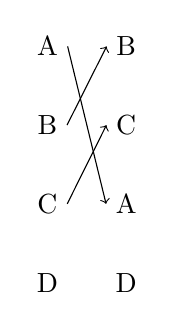
\begin{tikzpicture}
\node (a1) {A};
\node (b1) [below of = a1] {B};
\node (c1) [below of = b1] {C};
\node (d1) [below of = c1] {D};
\pause
\node (b2) [right of = a1] {B};
\node (c2) [right of = b1] {C};
\node (a2) [right of = c1] {A};
\node (d2) [right of = d1] {D};
\draw[->] (a1.east) -- (a2.west);
\draw[->] (b1.east) -- (b2.west);
\draw[->] (c1.east) -- (c2.west);
%\draw[->] (d1.east) -- (d2.west);
\pause
\end{tikzpicture}
\end{figure}
\onslide<5->{
\column{.3\textwidth}
\begin{figure}
\begin{tikzpicture}
\node (a1) {A};
\node (b1) [below of = a1] {B};
\node (c1) [below of = b1] {C};
\node (d1) [below of = c1] {D};}
\onslide<6->{
\pause
\node (a2) [right of = a1] {A};
\node (c2) [right of = b1] {C};
\node (b2) [right of = c1] {B};
\node (d2) [right of = d1] {D};
%\draw[->] (a1.east) -- (a2.west);
\draw[->] (b1.east) -- (b2.west);
\draw[->] (c1.east) -- (c2.west);
%\draw[->] (d1.east) -- (d2.west);
}
\onslide<7->{
\pause
\node (b3) [right of = a2] {B};
\node (c3) [right of = c2] {C};
\node (a3) [right of = b2] {A};
\node (d3) [right of = d2] {D};
%\draw[->] (a1.east) -- (a2.west);
\draw[->] (b2.east) -- (b3.west);
\draw[->] (a2.east) -- (a3.west);
%\draw[->] (d1.east) -- (d2.west);
%%FIXME: ADD NUMBERS HERE AND FIX TIMINGS SO THEY APPEAR WITH THE
%%CYCLE NOTATION
}
\pause
\end{tikzpicture}
\end{figure}
\column{.3\textwidth}
\onslide<8->{
In symbols:
$$ \left(\begin{tabular}{cccc}
1 & 2 & 3 \\
3 & 1 & 2 \\
\end{tabular}\right) = $$ $$ \left(\begin{tabular}{cc}
2 & 3 \\
3 & 2 \\
\end{tabular}\right)\circ\left(
\begin{tabular}{cc}
1 & 3 \\
3 & 1 \\
\end{tabular}\right)$$ $$ = (2\,3)\circ(1\,3)$$
\end{columns}
}
\onslide<9->{
Notice that the order of composition is important.}
\end{frame}

\begin{frame}
\frametitle{Grouping by addition}
\begin{itemize}
\item In usual arithmetic, addition is commutative: \pause $2+3=3+2$ \pause
\item We have seen that composition of permutations is \emph{not}
  commutative if they both move the same symbol:\pause
\begin{itemize}
\item $(1\,2)\circ(1\,3)=\left(\begin{tabular}{ccc}1 & 2 & 3\\ 2 & 3 &
      1\end{tabular}\right)$ but $(1\,3)\circ(1\,2)=\left(\begin{tabular}{ccc}1 & 2 & 3\\ 3 & 1 &
      2\end{tabular}\right)$ \pause
\end{itemize}
\item We can also ``add'' permutations without combining them: \pause
\begin{itemize}
\item  $(1\,2)+(1\,3)=(1\,3)+(1\,2)$
\pause
\end{itemize}
\item Now we can write expressions like
  $\left((1\,2)+(1\,3)\right)\circ(2\,3) $ \pause
\item We can work with this by \emph{distributing} the composition:
\end{itemize}
$((1\,2)+(1\,3))\circ(2\,3) = \pause (1\,2)\circ(2\,3) +
(1\,3)\circ(2\,3) = \pause \left(\begin{tabular}{ccc}1 & 2 & 3\\ 3 & 1 &
      2\end{tabular}\right) + \left(\begin{tabular}{ccc}1 & 2 & 3\\ 2 & 3 &
      1\end{tabular}\right) \pause \textcolor{red}{=
    (2\,3)\circ((1\,2)+(1\,3))}$
\begin{itemize}
\item Composition of these types of expressions is \emph{sometimes} commutative. 
\end{itemize}
\end{frame}

\begin{frame}
\frametitle{Graphs}
\begin{block}{Definition}
A \emph{graph} is a collection of points (called \emph{vertices}) and
lines connecting them (called \emph{edges}).
\end{block}
\pause
Examples: 
\begin{columns}
\column{.3\textwidth}
\begin{figure}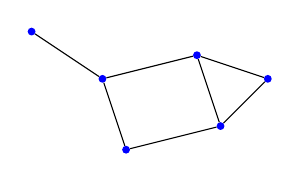
\begin{tikzpicture}
  [scale=.3,auto=left,every node/.style={circle,fill=blue,scale=.3}]
  \node (n6) at (1,10) {};
  \node (n4) at (4,8)  {};
  \node (n5) at (8,9)  {};
  \node (n1) at (11,8) {};
  \node (n2) at (9,6)  {};
  \node (n3) at (5,5)  {};

  \foreach \from/\to in {n6/n4,n4/n5,n5/n1,n1/n2,n2/n5,n2/n3,n3/n4}
    \draw (\from) -- (\to);

\end{tikzpicture}
\end{figure}
\begin{figure}
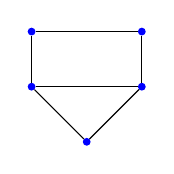
\begin{tikzpicture}
  [scale=.7,auto=left,every node/.style={circle,fill=blue,scale=.3}]
  \node (n1) at (2,1) {};
  \node (n2) at (1,2) {};
  \node (n3) at (3,2) {};
  \node (n4) at (1,3) {};
  \node (n5) at (3,3) {};

  \foreach \from/\to in {n1/n2,n1/n3,n2/n3,n2/n4,n4/n5,n5/n3}
    \draw (\from) -- (\to);

\end{tikzpicture}
\end{figure}
\column{.3\textwidth}
\begin{figure}
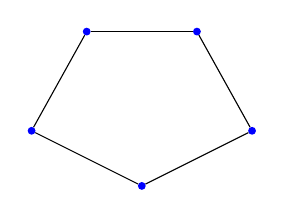
\begin{tikzpicture}
  [scale=.7,auto=left,every node/.style={circle,fill=blue,scale=.3}]
  \node (n1) at (3,1) {};
  \node (n2) at (1,2)  {};
  \node (n3) at (5,2)  {};
  \node (n4) at (2,3.8) {};
  \node (n5) at (4,3.8)  {};

  \foreach \from/\to in {n1/n2,n2/n4,n4/n5,n5/n3,n3/n1}
    \draw (\from) -- (\to);

\end{tikzpicture}
\end{figure}
\begin{figure}
\begin{tikzpicture}
  [scale=.3,auto=left,every node/.style={circle,fill=blue,scale=.3}]
  \node (n6) at (1,10) {};
  \node (n4) at (4,8)  {};
  \node (n5) at (8,9)  {};
  \node (n1) at (11,8) {};
  \node (n2) at (9,6)  {};
  \node (n3) at (5,5)  {};

  \foreach \from/\to in {n6/n4,n5/n1,n1/n2,n3/n4}
    \draw (\from) -- (\to);

\end{tikzpicture}
\end{figure}

\column{.3\textwidth}
\begin{figure}
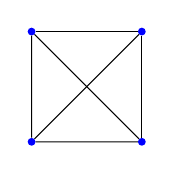
\begin{tikzpicture}
  [scale=1.4,auto=left,every node/.style={circle,fill=blue,scale=.3}]
  \node (n4) at (1,1) {};
  \node (n3) at (1,2)  {};
  \node (n2) at (2,1)  {};
  \node (n1) at (2,2) {};

  \foreach \from/\to in {n1/n2,n2/n3,n3/n4,n1/n4,n1/n3,n2/n4}
    \draw (\from) -- (\to);

\end{tikzpicture}
\end{figure}
\begin{figure}
\begin{tikzpicture}
  [scale=.2,auto=left,every node/.style={circle,fill=blue,scale=.3}]
  \node (n6) at (1,10) {};
  \node (n4) at (6,8)  {};
  \node (n5) at (8,9)  {};
  \node (n1) at (4,9) {};
  \node (n2) at (9,2)  {};
  \node (n3) at (5,5)  {};

\end{tikzpicture}
\end{figure}

\end{columns}

\end{frame}

\begin{frame}
\frametitle{Complete graphs} % And labellings
\begin{block}{Definition}
A \emph{complete graph} is a graph in which every vertex is joined to
every other vertex.\pause
\begin{columns}
\column{.5\textwidth}
\begin{figure}
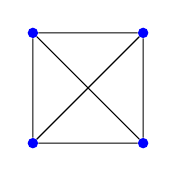
\begin{tikzpicture}
  [scale=1.4,auto=left,every node/.style={circle,fill=blue,scale=.4}]
  \node (n4) at (1,1) {};
  \node (n3) at (1,2)  {};
  \node (n2) at (2,1)  {};
  \node (n1) at (2,2) {};

  \foreach \from/\to in {n1/n2,n2/n3,n3/n4,n1/n4,n1/n3,n2/n4}
    \draw (\from) -- (\to);

\end{tikzpicture}
\end{figure}
\column{.5\textwidth}
\begin{figure}
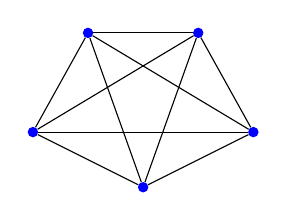
\begin{tikzpicture}
  [scale=.7,auto=left,every node/.style={circle,fill=blue,scale=.4}]
  \node (n1) at (3,1) {};
  \node (n2) at (1,2)  {};
  \node (n3) at (5,2)  {};
  \node (n4) at (2,3.8) {};
  \node (n5) at (4,3.8)  {};

  \foreach \from/\to in {n1/n2,n1/n3,n1/n4,n1/n5,n2/n3,n2/n4,n2/n5,n3/n4,n3/n5,n4/n5}
    \draw (\from) -- (\to);

\end{tikzpicture}
\end{figure}
\end{columns}
\end{block}
\pause

\begin{itemize}
\item We can also label the vertices:
\begin{figure}
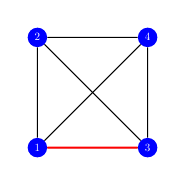
\begin{tikzpicture}
  [scale=1.4,auto=left,every node/.style={circle,color=white,fill=blue,scale=.4}]
  \node (n1) at (1,1) {1};
  \node (n2) at (1,2)  {2};
  \node (n3) at (2,1)  {3};
  \node (n4) at (2,2) {4};

  \foreach \from/\to in {n1/n2,n2/n3,n3/n4,n1/n4,n1/n3,n2/n4}
    \draw (\from) -- (\to);
  \only<4->{\draw[red,thick] (n1) -- (n3);}
\end{tikzpicture}
\end{figure}

\pause
\item This gives a way of representing transpositions: \only<4->{\textcolor{red}{$(1\,3)$}}
\end{itemize}

\end{frame}

\begin{frame}
\frametitle{Reformulating the problem}
\begin{itemize}
\item Our original problem was to find a way of grouping the
  transpositions together so that they commute.\pause
\item For three symbols (numbers, letters), there are three transpositions:
\begin{itemize}
\pause
\item Elements in the set $\{\textcolor<5->{red}{(1\,2)},\textcolor<5->{blue}{(1\,3)},\textcolor<5->{green}{(2\,3)}\}$ do not
  commute. %%FIXME TIME COLORS TO CORRESPOND TO THE GRAPHS
\item Elements in the set $\{\textcolor<5->{orange}{(1\,2)+(1\,3)},\textcolor<5->{purple}{(2\,3)}\}$ \emph{do} commute.
\end{itemize}
\pause
\item If the transpositions are represented by edges on a graph, then
  we can group them together by coloring them.
\end{itemize}
\pause
\begin{columns}
\column{.4\textwidth}
\begin{figure}
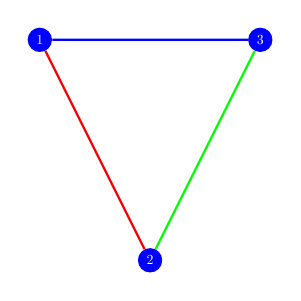
\begin{tikzpicture}
  [scale=1.4,auto=left,every node/.style={circle,color=white,fill=blue,scale=.5}]
  \node (n1) at (1,4) {1};
  \node (n2) at (2,2)  {2};
  \node (n3) at (3,4)  {3};

  \draw[thick,red] (n1) -- (n2);
  \draw[thick,green] (n2) -- (n3);
  \draw[thick,blue] (n3) -- (n1);

\end{tikzpicture}
\end{figure}

\column{.4\textwidth}
\begin{figure}
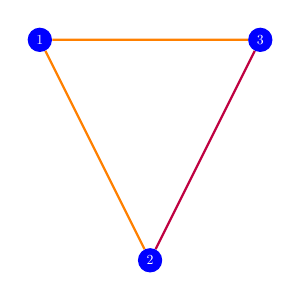
\begin{tikzpicture}
  [scale=1.4,auto=left,every node/.style={circle,color=white,fill=blue,scale=.5}]
  \node (n1) at (1,4) {1};
  \node (n2) at (2,2)  {2};
  \node (n3) at (3,4)  {3};

  \draw[thick,orange] (n1) -- (n2);
  \draw[thick,purple] (n2) -- (n3);
  \draw[thick,orange] (n3) -- (n1);

\end{tikzpicture}
\end{figure}

\end{columns}
\end{frame}

\begin{frame}
\frametitle{Gallai colorings}
\begin{block}{Definition}
An edge coloring of a complete graph is said to be \emph{Gallai} if no
triangles on the graph are drawn with three different colors. \pause
\end{block}
\begin{columns}
\column{.4\textwidth}
Examples:
\begin{figure}
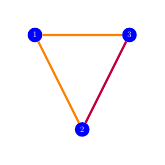
\begin{tikzpicture}
  [scale=.6,auto=left,every node/.style={circle,color=white,fill=blue,scale=.3}]
  \node (n1) at (1,4) {1};
  \node (n2) at (2,2)  {2};
  \node (n3) at (3,4)  {3};

  \draw[thick,orange] (n1) -- (n2);
  \draw[thick,purple] (n2) -- (n3);
  \draw[thick,orange] (n3) -- (n1);

\end{tikzpicture}
\end{figure}

\begin{figure}
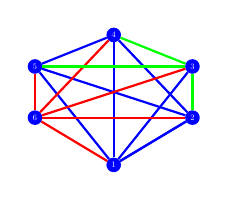
\begin{tikzpicture}
  [scale=.5,auto=left,every node/.style={circle,color=white,fill=blue,scale=.3}]
  \node (n1) at (2,.8) {1};
  \node (n2) at (4,2) {2};
  \node (n3) at (4,3.3) {3};
  \node (n4) at (2,4.1) {4};
  \node (n5) at (0,3.3) {5};
  \node (n6) at (0,2) {6};

  \draw[thick,blue] (n1) -- (n2);
  \draw[thick,blue] (n1) -- (n2);
  \draw[thick,blue] (n1) -- (n3);
  \draw[thick,blue] (n1) -- (n4);
  \draw[thick,blue] (n1) -- (n5);
  \draw[thick,blue] (n2) -- (n4);
  \draw[thick,blue] (n2) -- (n5);
  \draw[thick,blue] (n4) -- (n5);

  \draw[thick,red] (n6) -- (n1);
  \draw[thick,red] (n6) -- (n2);
  \draw[thick,red] (n6) -- (n3);
  \draw[thick,red] (n6) -- (n4);
  \draw[thick,red] (n6) -- (n5);

  \draw[thick,green] (n2) -- (n3);
  \draw[thick,green] (n3) -- (n4);
  \draw[thick,green] (n3) -- (n5);
\end{tikzpicture}
\end{figure}
\pause

\column{.4\textwidth}
Non-examples:
\begin{figure}
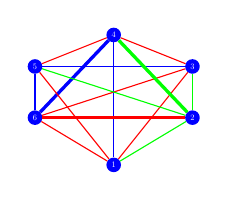
\begin{tikzpicture}
  [scale=.5,auto=left,every node/.style={circle,color=white,fill=blue,scale=.3}]
  \node (n1) at (2,.8) {1};
  \node (n2) at (4,2) {2};
  \node (n3) at (4,3.3) {3};
  \node (n4) at (2,4.1) {4};
  \node (n5) at (0,3.3) {5};
  \node (n6) at (0,2) {6};

  \draw[blue] (n3) -- (n5);
  \draw[very thick,blue] (n6) -- (n4);
  \draw[blue] (n6) -- (n5);
  \draw[blue] (n1) -- (n4);

  \draw[red] (n1) -- (n6);
  \draw[red] (n1) -- (n5);
  \draw[red] (n1) -- (n3);
  \draw[very thick,red] (n2) -- (n6);
  \draw[red] (n3) -- (n4);
  \draw[red] (n3) -- (n6);
  \draw[red] (n4) -- (n5);

  \draw[green] (n2) -- (n1);
  \draw[green] (n2) -- (n5);
  \draw[very thick,green] (n2) -- (n4);
  \draw[green] (n2) -- (n3);
\end{tikzpicture}
\end{figure}

\begin{figure}
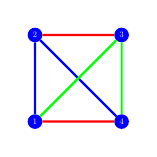
\begin{tikzpicture}
  [scale=1.1,auto=left,every node/.style={circle,color=white,fill=blue,scale=.3}]
  \node (n1) at (1,1) {1};
  \node (n2) at (1,2) {2};
  \node (n3) at (2,2) {3};
  \node (n4) at (2,1) {4};


  \draw[thick,blue] (n1) -- (n2);
  \draw[thick,blue] (n2) -- (n4);

  \draw[thick,red] (n1) -- (n4);
  \draw[thick,red] (n2) -- (n3);

  \draw[thick,green] (n1) -- (n3);
  \draw[thick,green] (n3) -- (n4);
\end{tikzpicture}
\end{figure}

\end{columns}
\end{frame}

\begin{frame}
\frametitle{Results}
\begin{block}{The Big Theorem}
A partition of the set of transpositions is commutative if and only if the corresponding graph is Gallai colored.
\end{block}
\pause

\begin{columns}
\column{.4\textwidth}
\begin{figure}
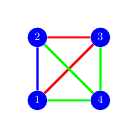
\begin{tikzpicture}
  [scale=.8,auto=left,every node/.style={circle,color=white,fill=blue,scale=.4}]
  \node (n1) at (1,1) {1};
  \node (n2) at (1,2) {2};
  \node (n3) at (2,2) {3};
  \node (n4) at (2,1) {4};

  \draw[thick,blue] (n1) -- (n2);

  \draw[thick,red] (n1) -- (n3);
  \draw[thick,red] (n2) -- (n3);

  \draw[thick,green] (n1) -- (n4);
  \draw[thick,green] (n2) -- (n4);
  \draw[thick,green] (n3) -- (n4);
\end{tikzpicture}
\end{figure}
\pause
\column{.5\textwidth}
$\{\textcolor{blue}{(1\,2)},$\\
$\textcolor{red}{[(1\,3)+(2\,3)]},$\\ 
$\textcolor{green}{[(1\,4)+(2\,4)+(3\,4)]}\}$
\end{columns}
\vspace{1cm}
\pause
\begin{columns}
\column{.4\textwidth}
\onslide<5->{
\begin{figure}
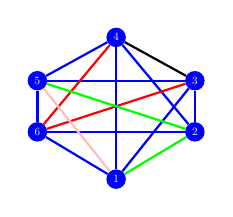
\begin{tikzpicture}
  [scale=.5,auto=left,every node/.style={circle,color=white,fill=blue,scale=.4}]
  \node (n1) at (2,.8) {1};
  \node (n2) at (4,2) {2};
  \node (n3) at (4,3.3) {3};
  \node (n4) at (2,4.4) {4};
  \node (n5) at (0,3.3) {5};
  \node (n6) at (0,2) {6};

  \draw[thick,blue] (n1) -- (n3);
  \draw[thick,blue] (n1) -- (n4);
  \draw[thick,blue] (n1) -- (n6);
  \draw[thick,blue] (n2) -- (n3);
  \draw[thick,blue] (n2) -- (n6);
  \draw[thick,blue] (n2) -- (n4);
  \draw[thick,blue] (n3) -- (n5);
  \draw[thick,blue] (n4) -- (n5);
  \draw[thick,blue] (n5) -- (n6);

  \draw[thick,red] (n3) -- (n6);
  \draw[thick,red] (n4) -- (n6);

  \draw[thick,green] (n1) -- (n2);
  \draw[thick,green] (n2) -- (n5);

  \draw[thick,pink] (n1) -- (n5);

  \draw[thick,black] (n3) -- (n4);
\end{tikzpicture}
\end{figure}}
\onslide<4->{
\column{.5\textwidth}
$\{\textcolor{blue}{[(1\,3)+(1\,4)+(1\,6)+(2\,3)}$\\
$\textcolor{blue}{+(2\,4)+(2\,6)+(3\,5)+(4\,5)+(5\,6)]},$\\
$\textcolor{red}{[(3\,6)+(4\,6)]},$\\ 
$\textcolor{green}{[(1\,2)+(2\,5)],}$\\
$\textcolor{pink}{(1\,5)},$\\
$\textcolor{black}{(3\,4)}\}$}
\end{columns}
\end{frame}

\begin{frame}
\frametitle{Schur rings}
We have given a partition on the set of transpositions that
commutes. What about other permutations?\pause
\begin{block}{Definition}
A \emph{Schur ring} or \emph{S-ring} is a similar partition on
\textbf{all} the permutations of a certain number of symbols.
\end{block}

\pause
\begin{itemize}
\item The classification of S-rings is an open research problem in
  modern algebra.\pause
\item Understanding the ways in which \emph{commutative} S-rings can be
  constructed would represent an important development.
\end{itemize}

\end{frame}
\begin{frame}
\Huge{\centerline{Thank you!}}
\end{frame}

%----------------------------------------------------------------------------------------

\end{document} 